\documentclass[12pt]{article}
\usepackage[utf8]{inputenc} % input encoding
\usepackage[T1]{fontenc} % Use an 8-bit font encoding, so that ã is a
                         % single glyph in the font. Yields better
                         % hyphenation and better cut-and-paste from pdf
\usepackage{times} % Comment this line you you want the default font, Computer Roman
% \usepackage[portuguese]{babel} % Uncomment this file you plan to write in Portuguese
\usepackage{hyperref}
\usepackage{listings}
\usepackage{graphicx}
\usepackage[section]{placeins}
\usepackage{multicol}
\usepackage{tabularx}
\usepackage{makecell}
\usepackage{amsmath}
\usepackage{tcolorbox}
\usepackage{float}
\graphicspath{ {./images/} }
\sloppy
\usepackage{geometry}

\lstset{frame=tb,
  aboveskip=3mm,
  belowskip=3mm,
  showstringspaces=false,
  columns=flexible,
  basicstyle={\small\ttfamily},
  numbers=none,
  breaklines=true,
  breakatwhitespace=true,
  tabsize=3
}

\title{Casual Language Documentation \\
  \Large Compiling Techniques 2019--2020
}
\author{
  João David\\49448
}
\date{26/06/2020}

\begin{document}
\maketitle


\section{Getting Started}
\subsection{Running the compiler}
The casualc script accepts as argument the casual source file that will be compiled and then creates a binary file with the same name of the source file (without the .cas). 

Since this language supports imports, all the source files involved in the process must be passed as argument, so that the compiler may link them and output a single binary file, that will have the name of the first source code passed as argument.

For instance, "casualc hello.cas math.cas util.cas" will output the binary hello.
From all the source files passed to the compiler, there must be exactly one defined method with the name "main". This will be the method executed first by the binary file.

\subsection{Example files}
The directory "./cas\_files" has several example casual files, ranging from basic var declaration, prints and matrix manipulation example files, to well known algorithms, such as fibonacci, quicksort and bubblesort.
Compile the files main.cas, file.cas and util.cas together to see the import functionality working.

\newpage
%-------------------------------------------------------------------------

\subsection{Syntax Highlighter}
The Casual Language has a syntax highlighter extension for Visual Studio Code. This tool also has auto-complete functionality, that can be used by pressing CTRL+SPACE after writing some characters, if there are any words previously written using those characters, they will appear (e.g. variable and function names).
The extension can be installed through the "casual-syntax-highlighter-0.0.1.vsix" file.\\

\begin{figure}[htb]
  	\centering
  	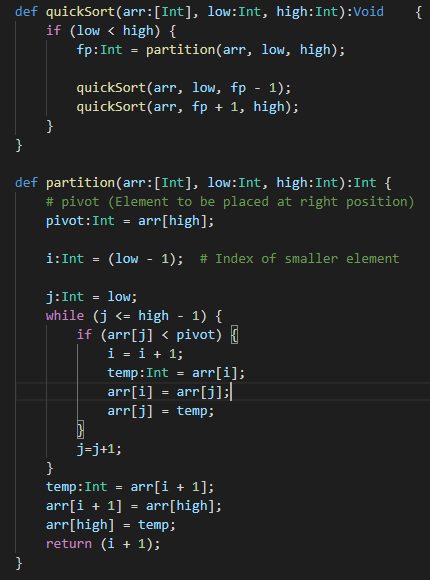
\includegraphics[scale=0.9]{quicksort.png}
\end{figure}
\newpage
%-------------------------------------------------------------------------

\section{Writing Casual code}
\subsection{Function declaration}
The Casual language has 12 built-in functions that can be used by the programmer, in order to use them, they have to be declared. The following list summarizes all existent declarable functions, they allow the user to print, create arrays, and matrixes for each data type (Int, Float, Bool and String). \\

\begin{itemize}
		\item decl printInt(i:Int):Void
        \item decl printFloat(f:Float):Void
        \item decl printBool(b:Bool):Void
        \item decl printString(s:String):Void
        \item decl new\_int\_array(n:Int):[Int]
        \item decl new\_float\_array(n:Int):[Float]
        \item decl new\_bool\_array(n:Int):[Bool]
        \item decl new\_string\_array(n:Int):[String]
        \item decl new\_int\_matrix(n:Int, m:Int):[[Int]]
        \item decl new\_float\_matrix(n:Int, m:Int):[[Float]]
        \item decl new\_bool\_matrix(n:Int, m:Int):[[Bool]]
        \item decl new\_string\_matrix(n:Int, m:Int):[[String]]       

\end{itemize}

\subsection{Import}
In order use the functions defined in an other casual file, use the import functionality by adding the import keyword followed by the casual file to be imported. For instance, "import util.cas". There must not be functions defined with equal names across all source files.

\newpage


\section{Implementation Decisions}
\subsection{Abstract Syntax Tree}
In the early stages of development of the compiler, the nodes within the AST did not store any information regarding types. This meant that, when validating the AST, the types were checked without storing the information in the AST. In the codegen phase, the types of the nodes were necessary to properly write the LLVM code according to the source code.

Since calculating the type of a certain node every time it was necessary would consume processor time, and it would repeat a computation previously done, the Visitor class that builds the AST was refactored in order to, whenever possible, store the type immediately, for instance, a function definition must always have the return type defined and as well as the types of the accepted parameters (var:type).

Some Node classes were refactored in order to have type setter and getter methods, the AST validator was also refactored in order to use those methods. Every time the type of a node was validated, the type was stored in the node using the setter.
For instance, the type of the root of the expression $3+4 <= 5*3$ would be set to Bool, and the roots of the expressions $3+4$ and $5*3$ would both be set to Int. Then, in the codegen phase, the getters were used to know the type of said expression and write the LLVM code accordingly.


\subsection{Linking Source files}
When passing more than one source file to the compiler, the type-checking must be done across all files, in order to verify that the functions invoked in a source file different from the one where they are defined, are respecting its signature. As well as, ensure that there are no function definitions with duplicate names across all source files.

The way the compiler does this is by creating an AST for each source file. When verifying each AST, the compiler starts by adding all the function definitions of the imported source files to the function context of the current AST validator, this way the compiler can type-check the function invocations within the current AST. The is done through the use of a HashMap where the key is the source file name, and the value the corresponding AST.

If no exceptions are raised, the compiler proceeds to create a new AST with all the functions defined and declared across all previous AST's (using aliasing), this new AST does not require to be validated, because this validation was done previously.

The codegen phase is done using this new AST, and the LLVM code is written to a single ".ll" file with the same name as the first source file passed as argument. Hence the importance of avoiding duplicate function names across all source files.

\newpage
%-------------------------------------------------------------------------

\subsection{Operator Precedence}

\textbf{Precedence order:} When computing the expression $3 + 3 * 5$, the operator with higher precedence goes first, in this case its the multiplication, the expression is  evaluated as if it was $3 + (3 * 5)$. 

\textbf{Associativity:} When an expression has two operators with the same precedence level, it is evaluated according to its associativity.  For instance, the expression $72 / 2 / 3$ is computed as if it was $(72 / 2) / 3$, because the division operator has left to right associativity. Some operators are not associative, therefore, they can't share the same operand with other operators in the same level of precedence. The expression $3 < 4 >= 4$ is invalid.

The following table summarizes all the information regarding precedence and associativity in Casual, a higher level means higher precedence.

\begin{table}[htb]
\centering
\begin{tabular}{| c | c | c | c |} 
 \hline
Level & Operator & Description & Associativity        \\ \hline
 9    & [ ]      & access array element & left to right \\ 
      & ( )      & parentheses          &  \\ \hline\hline
          
 8    & $- $     & unary minus          & right to left \\ 
      & $!$      & unary logical NOT    & \\ \hline\hline
      
 7    & $*$      &                      & \\ 
      & /        & multiplicative       & left to right \\
      & $\%$     &                      & \\ \hline\hline
      
 6    & $+$      & additive             & left to right\\
      & $-$      &                      & \\  \hline\hline
 
 5    & $< $     &                      & \\
      & $<=$     & relational           & not associative\\
      & $> $     &                      & \\
      & $>=$     &                      &  \\  \hline\hline 
      
 4    & $==$     & equality             & left to right\\
      & $!=$     &                      & \\ \hline\hline
      
 3    & $\&\&$   & logical AND          & left to right\\   \hline\hline
 
 2    & $||$     & logical OR           & left to right\\   \hline\hline
 
 1    & $=$      & assignment           & right to left \\   \hline
 
\end{tabular}
\end{table}
This precedence hierarchy was defined in the "expr" rule, within the ANTLR4 grammar, operators with a higher level of precedence were written above the ones with lower precedence level. For instance, if the rule "unary\_ope expr" was defined last, the expression $-3 + 5$ would result in $-8$ instead of $2$.

\newpage
%-------------------------------------------------------------------------

\subsection{Context type}
The process of validating an AST requires two types of Context data structures. Since Casual supports the invocation of functions defined after the function where the invocation takes place, it is mandatory to parse first through all function declarations and definitions. This information is stored in the FuncSignContext, within this class there is a hash-map where the key is the function name, and the value is the FuncSignatureScope, where the parameters type and return type are stored. This way, when a function is invoked inside a function definition block, the FuncSignContext is used to look for said function.

The second type of context was simply named Context, and it is responsible to control the scopes within a function definition, every time the AST validator enters an if then, if else or while blocks, a new scope is pushed into the stack of Scopes. Each Scope has a hash-map where the key is the variable name, and the value its type. This way it is extremely easy to know if a certain var name was already defined in previous scopes, and raise an exception if so. This is done by iterating over all Scopes within the stack.

Casual has a semantic similar to the one used in java, where a variable declared in a block, can't be declared again in nested blocks.

\subsection{Codegen}
The Casual built-in functions, described in the Function declaration subsection, were written in C, and then compiled to LLVM using clang. Every time the programmer declares those functions in the casual source file, the casual compiler will add them to the ".ll" file, that will then be compiled by the llc. If they are not declared, they won't be added to the ".ll" file.

All the instructions written into the ".ll" file in the codegen process, were also written with the help of auxiliary C files, this C files were written specifically with the purpose of understanding how LLVM handles certain instruction. This reverse engineer files can be found in the "./reverse\_eng\_files" directory.\\

The codegen phase uses the Emitter data structure, which has a stack of ScopeLLVM, each ScopeLLVM has a hash-map, where the key is the variable name in the casual source file, and the value is the variable name used in the LLVM code. Every time the codegenerator enters an if then, if else or while blocks, a new ScopeLLVM is pushed into the stack.
The emitter also has an int counter that is used to append to all names used in the LLVM file (variables, labels, etc). The value of the counter is incremented by one after each use, this way it is guaranteed to never exist repeated names within the LLVM file.\\

The nomenclature used for the while statement is while\_cond\_x for the guard, while\_body\_x for the while's block and while\_cont\_x for the statements after the while statement.
Regarding the if statement, they are then\_x for the then block, else\_x for the else block and cont\_x for the statements after the if statement. The x is the same for all labels regarding the same if or else statement. This way, when debugging the LLVM file, it is easier to understand which is which.

For variable names, the nomenclature is \%casVarName\_x, this way it is easier to identify the casual var name in the LLVM file.
For the rest of the intermediary operations, such as multiplication, function invocation, variable access, the LLVM names are self explanatory, for instance multiplication, subtraction, function invocation, equals are \%mul\_x, \%sub\_x, \%function\_call\_x and \%cmp\_eq\_x respectively.
The return is a special case, and has a \$ before the return word, in order to avoid conflicts with casual variable names, since it is impossible to declare variables in casual started by \$.

\bibliographystyle{plain}
\end{document}

%%% Local Variables:
%%% mode: latex
%%% TeX-master: t
%%% End:
